% IEEE Paper Template for US-LETTER Page Size (V1)
% Sample Conference Paper using IEEE LaTeX style file for US-LETTER pagesize.
% Copyright (C) 2006-2008 Causal Productions Pty Ltd.
% Permission is granted to distribute and revise this file provided that
% this header remains intact.
%
% REVISION HISTORY
% 20080211 changed some space characters in the title-author block
%
\documentclass[10pt,conference,letterpaper]{IEEEtran}
\usepackage{times,amsmath,epsfig}

\usepackage{subfigure}
\usepackage{color}
\usepackage{balance}  % for  \balance command ON LAST PAGE 
\usepackage{graphicx}
\usepackage{epstopdf}  % used for generating pdf 
\usepackage[english]{babel}
\usepackage[utf8]{inputenc}
\usepackage{amsmath}
\usepackage{graphicx}
\usepackage{caption}
% \usepackage[compress]{cite}
\usepackage[numbers,sort&compress]{natbib}
\renewcommand{\bibfont}{\footnotesize}
\usepackage{amsfonts} % for mathbb

\let\proof\relax
\let\endproof\relax
\usepackage{amsthm}


\usepackage{caption}
\usepackage{color}
\usepackage[ruled]{algorithm}
\usepackage{algorithmic}
\renewcommand{\algorithmiccomment}[1]{\bgroup #1 \egroup}




\newcommand{\ie}[0]{\textit{i.e.}}
\newcommand{\eg}[0]{\textit{e.g.}}
\newcommand{\etal}[0]{\textit{et al.}}


\newcommand{\keobf}{\textit{$(k,\epsilon)$-obf}}
\newcommand{\argmin}{\operatornamewithlimits{argmin}}
\newcommand{\genobf}{\texttt{\textbf{genObf}}}
\newcommand{\ere}{$\mathcal{E}RR-$eval}
\newcommand{\pg}{\mathcal{G}}
\newcommand{\Constraint}{$\mathcal{C}$}
\newcommand{\Number}{\|v\|}


\theoremstyle{plain}
\newtheorem{definition}{Definition}
\newtheorem{problem}{Problem}
\newtheorem{example}{Example}
\newtheorem{observation}{Observation}
\newtheorem{lemma}{Lemma}

\newcommand{\methodName}{Squid}
\newcommand{\soaName}{Obf}

\usepackage{enumitem}
\setlist[itemize]{leftmargin=2.5mm}


\title{Sharing Uncertain Graphs with Syntactic Anonymity}

% \author{Dongqing Xiao,  Mohamed Y. Eltabakh, Xiangnan Kong \\ 
% \affaddr{Worcester Polytechnic Institute (WPI), Computer Science Department, MA, USA} \\
% \{dxiao,~meltabakh,~xkong\}~@wpi.edu}  
\author{%
% author names are typeset in 11pt, which is the default size in the author block
{Dongqing Xiao, Mohamed Y. Eltabakh, Xiangnan Kong}%
% add some space between author names and affils
\vspace{1.4mm}\\
\fontsize{10}{10}\selectfont\itshape
Computer Science Department, Worcester Polytechnic Institute \\
Worcester, United States of America\\
\fontsize{9}{9}\selectfont\ttfamily\upshape
\{dxiao,~meltabakh,~xkong\}@wpi.edu\
}
\begin{document}
\maketitle


% NOTE keywords are not used for conference papers so do not populate them
% \begin{keywords}
% keyword-1, keyword-2, keyword-3
% \end{keywords}
%

\begin{abstract}  
Many graphs in real-world applications, such as social network and business to business network, are not deterministic but are uncertain. Related research requires open access to such uncertain graph datasets. While sharing these datasets often risks exposing sensitive data to the public. Current works mainly concern about privacy issues with deterministic graph sharing.  The uncertain scenario is overlooked. 

We first show conventional methods are not applicable for uncertain graph sharing. By disregarding the possible world semantic, they significantly disrupt the stochastic structure. Our work seeks a solution to share meaningful probabilistic graphs without compromising user privacy. We develop a syntactically private algorithm, Squid, for solving this problem. It integrates the possible world semantic into the core of anonymization. It enables a fine-grained, uncertainty-aware control over the injected noise. We apply our method to real uncertain graphs and show its efficiency and practical utility. 
% not only the statstics but also real-world applications 
\end{abstract}

\section{Introduction}

\label{sec:Intro}

% Graph-- Uncertain Graph--Examples 
Graphs are widely used to capture the complex relationships in emerging applications, such as business to business (B2B) and social networks. 
Sometimes, the existence of the relationship between two entities is uncertain. For instance, in social networks, nodes represents individual users, while edges represent friendship or trust link among them.  Usually, the link is derived by inference and prediction models built on interaction details~\cite{Lin_B2B,Adar_Managing_2007,Kempe_Maximizing_2003}. And, edge probability denotes the accuracy of a link prediction, or the trust of one person on another. 
In these applications, the data can be modeled and shared as uncertain graphs whose edges carries a probability of existence. The probability represents the confidence that the relationship holds in reality. 

\begin{figure}[!htb]
  \vspace{-7pt}
    \subfigure[Social Trust Network]{\label{fig:socialNetwork}
      \begin{minipage}[l]{0.46\columnwidth}
        \centering
        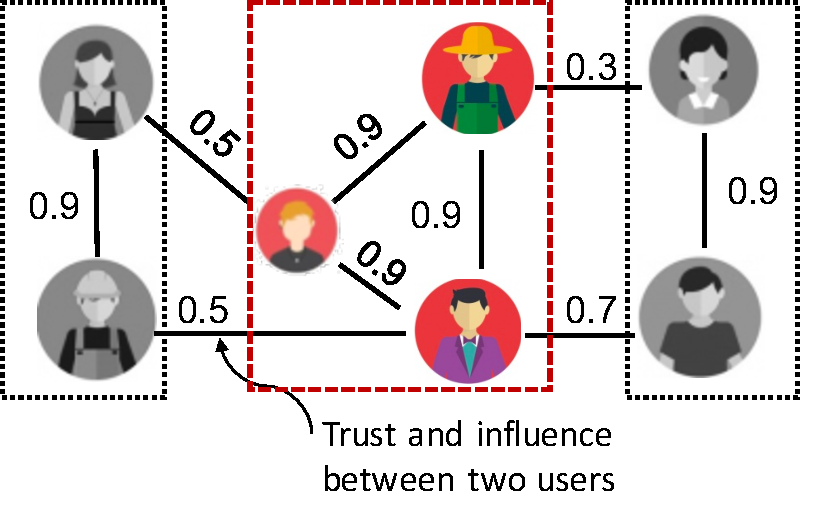
\includegraphics[height=2.7cm]{ill/SocialNetwork.pdf}
      \end{minipage}
      }
    \subfigure[B2B Network]{\label{fig:b2bNetwork}
      \begin{minipage}[l]{0.46\columnwidth}
        \centering
        \includegraphics[height=2.7cm]{ill/B2BNetwork.pdf}
      \end{minipage}
      }
    \vspace{-7pt}
    \caption{Real-world uncertain graphs with privacy concerns.}
    \label{fig:motivation}
    \vspace{-7pt}
\end{figure} 

% Sharing--Privacy--Examples 
These uncertain graphs are invaluable for scientific research and commercial applications~\cite{Kempe_Maximizing_2003,Cho_Friendship_2011}. However, sharing these uncertain graphs would violate the privacy of users or entities profiled inside. In social trust network, the trust relationships among users--- which greatly impact users' behaviors, are usually probabilistic.  They are useful in social interaction study and micro-targeting. While users are unwilling to share such confidential information with potential adversaries like Cambridge Analytica. In B2B networks, business operators also hesitate to share transaction patterns as it relates to  confidential business models. Such tension is raising the question of sharing uncertain graphs without compromising privacy. 


% State-of-Art 
A number of privacy preserving graph sharing schemes have been studied in the deterministic scenario~\cite{Liu_Towards_2008,Ying_Randomizing_2008,Wang2011,Liu_Privacy_2009,Nguyen_Anonymizing_2015,Sala_Sharing_2011,Xiao_Differentially_2014,lee2011}, though many problems still remain unexplored in the uncertain scenario.

\begin{figure}[!htb]
  \centering
  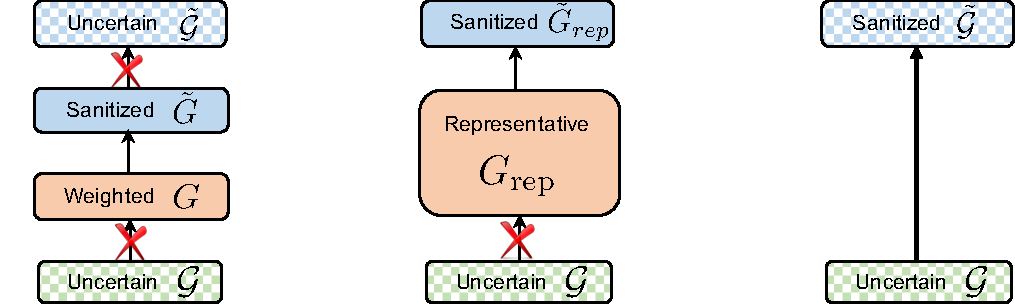
\includegraphics[width=0.9\linewidth]{ill/methods.pdf}
  \caption{XXXX.}
  \vspace{-14pt}
\end{figure}
%weight casting fails 
An obvious approach is to convert uncertain graph sharing problem into the deterministic case by casting edge probabilities as edge weights. 
Note that, one of the most important goals of sharing uncertain graphs is to maintain the data utility. 
However, by disregarding the possible world semantics of the uncertain graph, casting-based approach, as later illustrated, fails to reflect uncertain graph properties such as connectivity, dense subgraphs correctly~\cite{Zhao_Detecting_2014,Hua_Probabilistic_2010}. 
Hence, casting-based scheme could produce very poor result in the uncertain scenario even if the weighted graph anonymization algorithm is good. 

{\small Connectivity of deterministic subgraphs is generally measured by the concept of cut, which is defined as the sum of weights of intra edges. Generally, the bigger the cut, the harder to separate two subgraphs. In Figure~\ref{fig:motivation}(a), the equal cut $C(SG_{1},SG_{2})=C(SG_{3},SG_{2})=1$ implies the identical connectivity of $SG_{1}$ and $SG_{3}$ w.r.t $SG_{2}$. However, with the possible world semantics, we know the probability to separate $SG_{1}$ and $SG_{2}$ is $(1-0.5)^{2}=0.25$, and that to separate $SG_{2}$ and $SG_{3}$ is $(1-0.3)(1-0.7)=0.21$. Hence, in fact, $SG_{2}$ is closer to $SG_{1}$ than to $SG_{3}$.} 

Another approach proposed in our previous work~\cite{Xiao:2018}, called rep-based anonymization, is based on the idea of processing uncertain graph through representative instances~\cite{Parchas_Gullo_Papadias_Bonchi_2014}.
It first extracts a single deterministic representative instance $G$ that capture structural properties of the uncertain graph.
After that, anonymization can be then be proceed efficiently on $G$ using conventional algorithms, regardless of the uncertainty.  
However, Rep-An is is not always feasible. 
The detachment of edge uncertainty deteriorates the data utility. 

Conventional graph anonymization schemes are inadequate to share uncertain graphs with a desirable trade-off between privacy and utility. 
It is worthwhile to consider developing the specially optimized solution for handling following challenges. 

$\bullet$~\textup{\emph{Stochastic Privacy Attacks.}}~~Edge uncertainty plays an indispensable role in the uncertain graph model. It is impractical to discard them in the release.  
While the extra release of edge uncertainty makes privacy protection far more difficult as it empowers the adversary and makes the profiled entity more vulnerable. 
% To this end, we show the potential re-identification attack and present the corresponding solution. 

$\bullet$~\textup{\emph{Stochastic Utility Loss Metric.}}~~It is challenging to maintain the structure when the uncertain graph is modified to pursue anonymity. 
The structural distortion incurred is evaluated by the specially designed utility loss metric.  
It plays the key role in utility preserving. 
Unfortunately, existing graph utility loss metrics such as graph edit distance~\cite{Liu_Towards_2008}, spectrum discrepancy~\cite{Ying_Randomizing_2008}, community reconstruction error~\cite{Wang2011} and shortest path discrepancy~\cite{Liu_Privacy_2009} are not suitable in the uncertain scenario because of the ignorance of edge uncertainty.
% In this context, the discrepancy w.r.t standard uncertain graph reliability becomes a good criterion. It evaluates the connectivity difference in the context of the entire graph and meanwhile utilizes the possible world model. 

$\bullet$~\textup{\emph{Intractable Search Space.}}~~The goal is to find a sanitized graph with the desired level of privacy by as few graph mutations as possible. 
Even the simple deterministic graph anonymization problem, {\ie}, only with edge additions and deletions, is a NP-hard problem~\cite{Hartung_Theory_2015}. 
In the uncertain scenario, the edge modification is no longer a binary operation (addition/deletion), but can be infinite probability values. Exhaustive search is computationally intractable if the number of edges is large. 
This makes the problem of uncertain graph anonymization very challenging. 
 % Thus, we approximate the problem of interest via a randomized algorithm, which built on the basis of meta-heuristics. It excels in identifying a population of sanitized results with good quality.

In this work, we propose a solution tailored towards uncertain graphs via incorporating possible world semantics.  
It preserves as much the stochastic nature of the original uncertain graph as possible, while injecting enough structural noise to guarantee a chosen level of privacy.
Specifically, we make the following contributions.
\vspace{-5pt}
\begin{itemize}
\item We are the first to formulate the uncertain graph anonymization problem. 
 We show the potential re-identification attack and present the corresponding privacy notion. 
\item We propose an utility loss metric on the basis of reliability. It evaluates the connectivity difference in the context of the entire graph and also utilizes the possible world model. 
\item We propose a randomized algorithm with the hybrid of uncertainty-aware heuristics. It excels in identifying a population of sanitized results with good quality efficiently.
\item We conduct extensive experimental studies to demonstrate efficiency and practical utility of our algorithms.
\end{itemize}

The rest of the paper is organized as follows. In Section 2, we summarize related works and clarify our distinct privacy goal. In Section 3 we formulate the uncertain graph-anonymization problem. Sections 4 – 5 consider the anonymization problem in the context of uncertain graphs.  In Section 6 we apply our method to several real-world uncertain graphs, and demonstrate their efficiency and practical utility. 


\section{Related Works}
A significant amount of prior work has been done on protecting the privacy of network datasets.
The comprehensive survey is out of the scope of this paper. 
Here, we briefly summarize the related works and clarify our privacy goal. 

\textbf{Syntactic Privacy.}~~Early works on privacy-preserving network publishing (PPNP) focus on developing anonymization techniques. Many of them modify the graph structure in subtle ways that guarantee privacy but keep much of graph structure. The released graph is available for graph analysis tasks. These approaches provide privacy protection against specific de-anonymization attacks. Most of them leverage syntactic privacy models derived from $k$-anonymity~\cite{Sweeney:2002:KAM:774544.774552}. It requires creating $k$ identical neighborhoods, or $k$ identical degree nodes to blend victims. 

Corresponding graph anonymization methods can be classified into four main categories: (1) Clustering-based generalization~\cite{Hay_Anonymizing_2007,Bhagat_Class_2009,hay2010resisting}; (2)~{\em Edge modification}~\cite{Liu_Towards_2008, Zhou_Preserving_2008, Wang2011, Wu_k_2010, Skarkala_Privacy_2012}, 
(3)~{\em Edge randomization}~\cite{Liu_Privacy_2009,Ying_Randomizing_2008, Ninggal_Utility_2015},
and~(4)~{\em Uncertainty semantic-based modifications} which add uncertainty to some edges and thus converting the deterministic graph to an uncertain version~\cite{Boldi_Injecting_2012, Nguyen_Anonymizing_2015}. The uncertainty semantic-based approaches are known as the state-of-art ones because of their excellent privacy-utility trade-off, brought by the fine-grained perturbation leveraging the uncertain semantics. 

 
\textbf{Differential Privacy.}~~Another option is to apply {$\epsilon$}-differential privacy policy to providing privacy guarantee. It roughly falls into two directions. The first direction aims to release certain differentially private mining results, such as degree distributions, sub-graph counts, and frequent graph patterns~\cite{Xiao_Differentially_2014,Day:2016}. These methods only release query result, early uses of the data can affect the quality of later uses. What's worse, no new queries can be permitted on the data. The second direction aims to share the meaningful graph~\cite{Sala_Sharing_2011}. Most research in this direction projects an input graph to dK-series and ensures differential privacy on dK-series statistics. Later, private statistics are then either fed into generators or MCMC process to generate a fit synthetic graphs. While current techniques are still inadequate to provide desirable data utility for many graph mining tasks. 

\emph{All the methods target at providing privacy guarantee to the deterministic graph. The uncertain scenario is overlooked.}
\vspace{-5pt}
\subsection{Our Privacy Goal}
Our work seeks a solution to share meaningful uncertain graphs while preserving privacy.
As ever discussed, existing PPNP schemes fail to provide utility guarantee in the uncertain scenario. 
We believe the anonymization process needed to be specially optimized. 
In this paper, we try to move this line of research one step forward from the deterministic context to a broader probabilistic context.

There is a widespread belief that differential privacy and its offsprings are immune to various privacy attacks. It offers a guarantee bound $\epsilon$ on the loss of privacy due to the data release~\cite{Sala_Sharing_2011,Xiao_Differentially_2014}. However, there is no clear way to set a general policy for choosing the privacy parameter $\epsilon$ for sufficient privacy guarantee~\cite{lee2011}. Its implications and impacts on the risk of disclosure in practice heavy depends on data detail. Thus, differential privacy is difficult to apply in practice. 

In contrast, the notion of syntactic privacy can generally be defined and understood based on the data schema. And, its parameters have a clear privacy meaning that can be understood independent of the actual data. Moreover, they have a clear relationship to the privacy regulation of individual identifiability (e.g., European GDPR Law). 
Hence, we focus on sharing uncertain graphs with syntactic anonymity in this work. 




\section{Problem Formulation}
\label{sec:notation}

% In this section, we provide background on uncertain graph, motivate the basic privacy attack, and formulate the uncertain graph anonymization problem. 
In this section, we provide background on uncertain graph, privacy attack and justify our choice of utility loss metric. 
On this basis, we present our formulation of the uncertain graph anonymization problem. 

\vspace{-4pt}
\subsection{Uncertain Graph}
\vspace{-2.5pt}
An uncertain graph $\mathcal{G}=(V,E,\mathit{p})$, is defined over a set of nodes $V$, a set of edges $E$, and a set of probabilities $\mathit{p}$ of edge existence. Following the literature~\cite{Potamias_K_2010,Zhao_Detecting_2014,Colbourn_Colbourn_1987}, we assume possible-worlds semantics, and we consider the edge probabilities independent~\footnote{We leave the conditional probability model as a future
extension.}. An uncertain graph $\mathcal{G}=(V,E,\mathit{p})$ essentially represents a probability distribution over all of the certain graphs $G$ in the forms of which the uncertain graph may actually exist. 
The probability of observing any possible world $G_i=(V,E_{G_i})$ is    
\begin{equation*}
    Pr[G_i]=\prod_{e \in E_{G_i}} {\mathit{p}(e)} \prod_{e \in E \setminus E_{G_i}} 1-\mathit{p}(e)
\end{equation*}

\subsection{Privacy Attack}
\label{sec:AMPC}
\vspace{-5pt}
\begin{figure}[!htb]
  \vspace{-10pt}
    \subfigure[Social Trust Network]{\label{fig:socialNetwork}
      \begin{minipage}[l]{0.46\columnwidth}
        \centering
        \includegraphics[height=2.7cm]{ill/example_source.pdf}
      \end{minipage}
      }
    \subfigure[The naive anonymization]{\label{fig:b2bNetwork}
      \begin{minipage}[l]{0.46\columnwidth}
        \centering
        \includegraphics[height=2.7cm]{ill/example_output.pdf}
      \end{minipage}
      }
    \vspace{-7pt}
    \caption{The Structural Re-Identification Issue.}
    \label{fig:privacyAttack}
    \vspace{-7pt}
\end{figure} 
Apparently, simply removing the identities of the nodes before publishing the uncertain graph does not guarantee privacy.  The structure of the uncertain graph itself, and in its basic form the degree of the nodes, can be revealing the identities of individuals. 
In practice, the adversary may have access to external information about the entities in the graphs. This information may be obtained by the adversary's malicious actions. 
For example, for the uncertain graph in Figure~\ref{fig:privacyAttack}, the adversary might know that ``Fred has three or more \textbf{trust} neighbors''. Such information allows the adversary to narrow down the set of candidates in the sanitized graphs. For example, the statement partially re-identify Fred as $\lbrace 2,3,6 \rbrace$ with \textbf{probabilities} respectively. 
Different to the deterministic scenario,  there are different posterior probabilities over candidate nodes $\lbrace 2,3,6 \rbrace$ where $P(6|\text{Fred}) \simeq P(3|\text{Fred}) \gg P(2|\text{Fred})$.

The node is vulnerable to the re-identification risk. Entity Re-identification (ER) can lead to additional disclosures. In this paper, we focus on the ER attack as this attack is one of the most serious privacy problems. 

\vspace{-12pt}
\subsection{Privacy Notion}
\label{sec:privacyNotion}
To resist re-identification attacks, we adopt the $(k,\epsilon)$-obf, an syntactic privacy notion,
% introduced by Boldi {\etal}~\cite{Boldi_Injecting_2012},
 where $k \ge 1$ is a desired level of obfuscation  and $\epsilon \ge 0$ is a tolerance parameter. 

\textsc{Obfuscation Parameter}~~Similar to $k-$anonymity, $k-$obf requires blending every entity with other fuzzy matching entities. While, the level of obfuscation is quantified as the entropy over posterior probabilities over fuzzy matching ones. It lower bounds the entropy of the distribution by $\log_{2} k$. 
\emph{Though it is initially used to measure the anonymity provided by an uncertain graph to the deterministic graph, the stochastic nature makes it a good fit in the uncertain scenario.} 

\textsc{Tolerance parameter}~~As for the tolerance parameter $\epsilon$, it serves for the following purpose. There might be extreme unique nodes, e.g., Trump in a Twitter network, whose obfuscation is almost impossible. Thus, Boldi {\etal}~\cite{Boldi_Injecting_2012} introduce a tolerance parameter $\epsilon$, which allows skipping up to $\epsilon * |V|$ nodes and makes the privacy goal more practical. 

% The formal definition is,
% \theoremstyle{definition}
% \begin{definition}
% 	\textbf{\boldmath{$(k,\epsilon)$}-obf \cite{Boldi_Injecting_2012}}
%     Let $P$ be a vertex property (i.e., vertex degree in our work), $k \geq 1$ be a desired level of anonymity, and $\epsilon >0 $ be a tolerance parameter. 
%     An sanitized uncertain graph $\tilde{\mathcal{G}}$ is said to $k$-obfuscate a given vertex $v \in \mathcal{G}$ w.r.t $P$ if the entropy $H()$ of the distribution $Y_{P(v)}$ over the nodes 
%     of $\tilde{\mathcal{G}}$ is greater than or equals to $\log_{2}{k}$:
%     \begin{equation*}
%         H(Y_{P(v)}) \geq \log_{2}{k}.
%     \label{obfCon}
%     \end{equation*}
% The uncertain graph $\tilde{\mathcal{G}}$
% is $(k,\epsilon)$-obf w.r.t property $P$ 
% if it $k$-obfuscates at least $(1-\epsilon)|V|$ nodes in $\mathcal{G}$. 
% \label{def:obf}
% \end{definition} 
\vspace{-12pt}
\subsection{Utility Loss Metric: Reliability Discrepancy}

As a fundamental property, connectivity plays a vital role in graph mining tasks such as nearest neighbor locating and clustering. 
The connectivity model can yield a better graph representation than the degree sequence model. 
Motivated by the above, connectivity discrepancy is widely used to measure the structural difference between deterministic graphs. 

The concept of reliability generalizes the connectivity concept uncertain scenario. 
It captures the probability that two given nodes are reachable over all possible worlds, as shown in Def~\ref{d:reliability}. 
Analogous to the deterministic case, we use reliability discrepancy as the utility-loss metric in the uncertain scenario, as outlined in Def~\ref{d:RD}. 
\begin{definition}
    \textbf{Two-Terminal Reliability~\cite{Colbourn_Colbourn_1987}}~~Given an uncertain graph $\mathcal{G}$, and two distinct nodes $u$ and $v$ in the graph, the reliability of $(u,v)$ is defined as:
        \begin{equation*}
                R_{u,v}(\mathcal{G})= \sum_{G \in W(\mathcal{G})} \mathcal{I}_{G}(u,v) ~ Pr[G] 
        \end{equation*}
    where $\mathcal{I}_{G}(u,v)$ is 1 iff $u$ and $v$ are contained in a connected component in $G$, and 0 otherwise.   
    \label{d:reliability}
\end{definition}

\theoremstyle{definition}
\begin{definition}
    \textbf{Reliability Discrepancy (RD)}
    The reliability difference between a sanitized output $\tilde{\mathcal{G}}$ and the original input $\mathcal{G}$, 
    denoted as $\Delta(\tilde{\mathcal{G}})$, 
    is defined as the sum of the two-terminal reliability discrepancy over all node pairs $(u,v) \in V_\mathcal{G}$.
    \begin{equation*}
        \Delta(\tilde{\mathcal{G}})=\sum_{(u,v) \in V_\mathcal{G} }|R_{u,v}(\mathcal{G})-R_{u,v}(\tilde{\mathcal{G}})|
    \end{equation*}
    \label{d:RD}
\end{definition}

\subsection{Problem Statement} 
% \vspace{-5pt}
\begin{problem}
     Given an uncertain graph $\mathcal{G}$ and desired anonymization parameters $k$ and $\epsilon$, 
     the objective is to find a  $(k,\epsilon)$-obf uncertain graph $\tilde{\mathcal{G}}$
     with the minimal utility loss,
     \vspace{-5pt}
     \begin{equation*}
             \begin{aligned}
                 & \argmin_{\tilde{
                \mathcal{G}}} & & \Delta(\tilde{\mathcal{G}}) \\
                &  \text{Subject to} & &\tilde{\mathcal{G}} \text{~is~} (k,\epsilon)-obf
            \end{aligned}
     \end{equation*}
     \label{prob:unobf}
\end{problem}
% add one paragraph to ....
\section{The State-of-Art Approach}
Before presenting our solution {\methodName} for uncertain graph sharing, we first describe the state-of-art approach ({\soaName})~\cite{Boldi_Injecting_2012}. 
The main purpose of describing it is to separate the basic framework with the key idea of {\methodName}. 
They differ in how they represent the graph property and how they perform mutation. 

\subsection{Overview}~~
The {\soaName} method obfuscates the (deterministic) graph data by adding or removing edges \emph{partially}. 
For each edge $e$, it assigns a probability deviation $r_{e}$, where $r_{e} \leftarrow R(\sigma)$. 
In particular, the uncertainty injecting scheme proceeds as follows:
\begin{equation}
	p(e) =
	\begin{cases}
		 1-r_{e}  & e \in E \\
		 r_{e}    & otherwise 
	\end{cases}
	\label{eq:inject}
\end{equation}

The most widely known member of generating distribution $R_{\sigma}$ is the truncated normal distribution with mean 0 and variance $\sigma^2$. 
While, $R$ could in principle be any distribution. 
As the standard deviation $\sigma$ decreases, a greater mass of $R_{\sigma}$ will concentrate near $r_{e}=0$.  
Then, the amount of injected noise and consequent structural distortion will be smaller. 
Aiming at high utility, {\soaName} aims at injecting the minimal amount of uncertainty need to achieve the required obfuscation. 
Thus, it calibrates the minimal amount of uncertainty via a binary search on the value of standard deviation $\sigma$, as outlined in Algorithm~\ref{alg:obf}.  
\vspace{-5pt}
\begin{algorithm}
{\scriptsize
	\begin{algorithmic}[1]
    	\item[] {\textbf{Input:}~Graph $\mathcal{G}$, obfuscation level $k$, tolerance parameter $\epsilon$}
        \item[] {\textbf{Output:}~The result $\mathcal{G}_{obf}$}
     	\STATE {$\sigma_{l} \leftarrow 0$; $\sigma_{u} \leftarrow 1$} \\
        \REPEAT
        \STATE{$\langle \hat{\epsilon}, \hat{\mathcal{G}} \rangle$ $\leftarrow$ \textbf{genObf}(-,$\sigma_{u}$)} \\
        \STATE{{\bf if} $\hat{\epsilon}=1$ (fail) {\bf then} $\sigma_{l} \leftarrow \sigma_{u}$; $\sigma_{u} \leftarrow 2\sigma_{u}$}
        \UNTIL{$\hat{\epsilon} \neq 1 $} \\
        \REPEAT
        	\STATE {$\sigma_{mid} \leftarrow (\sigma_{u}+\sigma_{l})/2$}
            \STATE{$\langle \hat{\epsilon}, \hat{\mathcal{G}} \rangle$ $\leftarrow$ \textbf{genObf}(-,$\sigma_{mid}$)}
            \STATE {{\bf if} $\hat{\epsilon} =1$~{\bf then}~$\sigma_{l} \leftarrow \sigma_{mid}$}\\
            \STATE {{\bf else} $\sigma_{u} \leftarrow \sigma_{mid}$;~~{$\mathcal{G}}_{obf} \leftarrow \hat{\mathcal{G}}$}
        \UNTIL{$\sigma_{u}-\sigma_{l}$ is enough small}
        % \COMMENT{\textcolor{blue}{\scriptsize Binary search for better obfuscation}}
        \STATE {return $\mathcal{G}_{obf}$}
    	\caption{The obfuscation algorithm}
	 \label{alg:obf}
    \end{algorithmic}
    }
\end{algorithm}
\vspace{-7pt}


The search flow is determined by the function {\genobf}. The function {\genobf} handles the search of {\keobf} instances using a given standard deviation parameter $\sigma$. It either returns the found {\keobf} instance or failure signals.
The search starts with an initial guess of an upper bound $\sigma_{u}$, which is iterative doubled until a {\keobf} instance is found. Then, the binary search is performed over the range $[0,\sigma_{u}]$. The binary search terminates until the search interval is sufficiently short. The algorithm outputs the best {\keobf} found (the last one that was successfully generated).

\subsection{The function {\genobf}}
In reality, finding {\keobf} instances using a given parameter $\sigma$ is not that easy.
The function {\genobf} utilizes the randomized search to handle intractable search space. Multiple attempts are performed (In our experiment, 5 attempts are performed.). Iff all the attempts fail, {\genobf} returns failure signals, otherwise, returns the found {\keobf} instance. 

Each attempt begins by selecting a subset of edges subject to alteration. Then, it assigns the deviation among selected edges and injects uncertainty. 
% The randomization process heavily relies on a single meta-heuristic. 
In particular, they suggest calibrating the perturbation applied to an edge $e$ according to the ``uniqueness" of the two nodes $u$ and $v$. 
% The calculation of uniqueness is covered in a sequent section. 
In brief, if both $u$ and $v$ are common nodes w.r.t the property, then $r_{e}$ should be very small; on the other hand, if $u$ and $v$ are outliers, then $r_{e}$ should be higher. Meanwhile, edges need to be sampled with the higher probability if they are adjacent to outliers. 


\subsection{Limitations} 
The above-mentioned approach achieves the desired level of obfuscation with the small change in the data, thus maintaining high utility 
However, the design heavily tailored towards the deterministic context. In the uncertain scenario, it suffers from following issues. 
First, its scheme does not consider the structural relevance of edges in critical edge selection/alteration steps, which leads to unnecessary structural distortion. 
Second, its scheme assumes the existence of edges is known with certainty, thus fails to handle uncertain graphs where the existence of edges is probabilistic. 
All the operators, such as selection and alteration, need to be integrated with possible world semantics carefully.  
We are left asking the question, \emph{how to generalize existing methods to the probabilistic context?}




\section{Privacy Via {\methodName}}
In this section we describe our algorithm, {\methodName}, which injects uncertainty to the given uncertain graph so that it becomes {\keobf} while preserving as much the stochastic nature as possible. A key feature of our method is to seamlessly integrate edge uncertainty and possible world semantics into the core of anonymization operators. 
% 
\subsection{Heuristic for Edge Perturbation}

% It is non-trivial to figure out the optimal set of edges that balances privacy gain and structural distortion. 
Selecting the set of edges subject to modification which balances privacy gain and structural distortion is 
a key component of graph anonymization. 
It involves consideration over the exponential number of edge combinations. 
Recently, the most popular paradigm for solving such problems has been using a class of heuristics. 
Successes of this approach include
(1) anonymity-aware ones that suggest injecting more considerable noise to unique nodes~\cite{Ying2009,Boldi_Injecting_2012,Hay_Anonymizing_2007} 
(2) utility-aware ones that indicate avoiding distortion over “bridge” edges whose deletion/addition would significantly impact the graph structure~\cite{Wang2011,Ninggal_Utility_2015}. 
The judicious edge selection must involve two types of heuristics which complement each other. 
Individually, they are far less effective. 
Nevertheless, they have not been explored yet in the context of uncertain graphs.

Motived by the above, we first generalize the calibration of uniqueness via the use of KL-divergence. 
Second, we propose a generalized edge relevance criterion from an information-theoretic perspective.
Besides, we develop an efficient algorithm for its computation in the context of uncertain graphs.
And, we show the use of such a criterion boosts XXX efficiently and straightforwardly.

\subsubsection{Generalized Uniqueness}

\begin{figure}
	\centering
        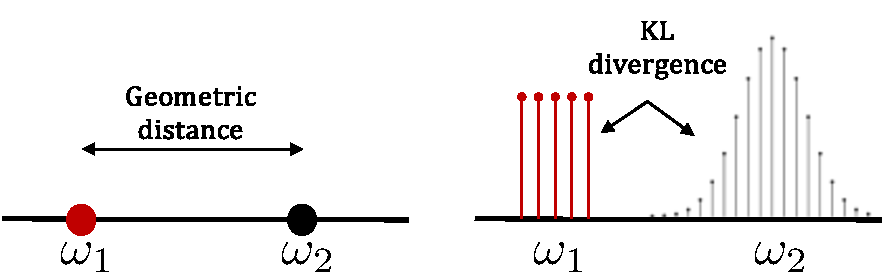
\includegraphics[width=\linewidth]{ill/shift_distance.pdf}
    \caption{Deterministic values and stochastic values.}
\end{figure}
The uniqueness criterion was used to measure how unique a given node is among all the nodes in the graph w.r.t a specific property. 
For a given node, its uniqueness score is the inverse of the commonness score of its property value $w$.
While, the commonness score of $w$ amounts to the weighted average distance among all other property values. 

The conventional method merely formulates node properties as discrete values and relies on the geometric distance function to measure their distance.  
Thus, it fails to handle our problem where the property values are stochastic.   
In this work, we extend the preliminary version for handing the stochastic case. 
We consider the use of probability distributions, which are essential characteristics of uncertain property values, in the measuring similarity between uncertain property values. 
We systematically model uncertain property values in both continuous and discrete domains as continuous and discrete random variables, respectively.
We use the well known Kullback-Leibler divergence to measure the distance between random variables with parameterized distributions. 
The generalized version of uniqueness score can then be formalized as
\begin{definition}
    \textbf{Uniqueness Score}
     Let $P:V \rightarrow  \Omega_{P}$ be a property on the set of nodes $V$ of the uncertain graph, 
     let $d$ be a KL divergence function, and let $\theta >0$  be a parameter. 
  	 Then the $\theta-$commonness of the property values $\omega$
  	 is $C_{\theta}(\omega):= \sum_{u \in V} \Phi_{0,\theta}(KL(\omega, P(v)))$,   
	 while the corresponding uniqueness is $U_{\theta}:= \frac{1}{C_{\theta}(\omega)}$. 
	 \vspace{-2pt}
\end{definition} 
Note that, the weights decays exponentially as a function of the KL divergence, 
and the parameter $\theta$ determines the decay rate. 
We set $\theta=\sigma$ as the injected noise blurs the meta distribution of property values. 
 
\subsubsection{Generalized Edge Relevance}

It is clear that alteration over a single edge would produce local structural change and send ripples through the rest of the graph. 
The incurred structural distortion varies on the topological role of the edge subjecting to alteration, even with the same amount of alteration. 
% Observe that edges with different roles will incur significantly different structural changes even with the same amount of injected noise. 
Targets at the high utility, we should penalize modification over structurally critical edges.  
Thus, we need measure the edge relevance w.r.t graph structure. 

There are many potential ways to measure it. 
Importantly, the metric must be fitted to the context of uncertain graphs.
Inspired by the concept of cut-edge, we measure the edge relevance of a given edge $e$
as the amount of structural distortion, measured by reliability discrepancy, caused by the unit noise subjects to the edge $e$, as follow. 
\begin{equation*}
    \mathcal{ERR}({e}) = \lim_{r_{e} \rightarrow 0} \frac{\Delta(\mathcal{G}+r_{e})}{r_{e}} 
                      = \sum_{u,v} \frac{|R_{u,v}(\mathcal{G}+r_{e}) -R_{u,v}(\mathcal{G})|} {r_{e}}
\end{equation*}

In deterministic graphs, a cut-edge of a graph is an edge whose deletion increases the number of connected components. 
In probabilistic graphs, $\mathcal{ERR}$ is used to generalize this concept by quantifying the stochastic impact of adding/deleting edge partially over the connectivity of all the possible worlds.
while the cut-edge is a binary classification, the $ERR$ value lies in the continuous range, and quantify the probability if the connected pairs holds in a possible world. 

In order to explore this point further, we have illustrate a probabilistic graph in Figure~\ref{}. 

% switch into the lemma format 
% The factorization lemma~\cite{Jin_Distance_2011} indicates
% \begin{align*}
%     R_{u,v}(\mathcal{G}+r_{e}) -R_{u,v}(\mathcal{G}) = r_{e} \cdot \big[ R_{u,v}(\mathcal{G}_{e})-R_{u,v}(\mathcal{G}_{\hat{e}}) \big]
% \end{align*}
% Then, the edge relevance $\mathcal{ERR}$ can then formulate as
% \begin{equation*}
%     \mathcal{ERR}(e) = \sum_{u,v} R_{u,v}(\mathcal{G}_{e}) \big- \sum_{u,v} R_{u,v}(\mathcal{G}_{\bar{e}})
% \end{equation*}

Observe that, $\mathcal{ERR}(e)$ amounts to the number difference of connected node pairs between two neighbor uncertain graphs $\mathcal{G}_{e}$ and $\mathcal{G}_{\bar{e}}$, 
where $\mathcal{G}_{e}$ and $\mathcal{G}_{\bar{e}}$ are identical to $\mathcal{G}$ with the exception that $p(e)=1$ in the former and $p(e)=0$ in the later. 





% We also show its computation can be achieved via Monte-Carlo sampling with an acceptable time complexity $\mathcal{O} (N \cdot T)$, where $N$ is the number of samples and $T$ is time complexity for the employed connected component detection algorithm.~\footnote{ The union-and-find method is used in this work.} The key idea is to memorize the calculated result (\# of connected node pairs) over samples. For each edge $e$, we group then aggregate results of samples according to edge existence. And, the vertex reliability relevance $\mathcal{VRR}$ amounts to the weighted sum of $\mathcal{ERR}$ values.












\input{squid_ex/exp.tex}
\input{conclusion.tex}
\bibliographystyle{abbrvnat}
% \bibliographystyle{abbrv}
\bibliography{refs}

\end{document}
